\documentclass{report}

%Russian-specific packages
%--------------------------------------
\usepackage[labelsep=space]{caption} [2022/02/20]
\usepackage{ltablex,booktabs}
\usepackage[english,russian]{babel}
\usepackage{fontspec}
\usepackage{indentfirst}
\usepackage{minted}
\setmainfont{Times New Roman}
\usepackage{enotez}
\setenotez{backref = true,list-heading ={\section{#1}} }
\DeclareTranslation{russian}{enotez-title}{Список литературы}
\usepackage{ulem}
\usepackage{listings, listings-rust}
\usepackage{amsmath}
\usepackage{graphics}
\usepackage{graphicx}
\usepackage{wrapfig}
\usepackage{textcomp}
\usepackage{lipsum}
\usepackage{xcolor}
\usepackage[document]{ragged2e}
\usepackage{longtable}
\usepackage{layout}
\usepackage[right=1.0in, left=1.0in, top=121pt, bottom=1.0in]{geometry}
\usepackage{fancyhdr}
\usepackage{capt-of}
%\usepackage[skip=10pt plus1pt, indent=40pt]{parskip}
\pagestyle{fancy}
\renewcommand{\baselinestretch}{1}
\fancypagestyle{plain}{%
    \fancyhf{} % clear all header and footer fields
    \fancyhead{} % clear all header fields
    \fancyfoot{} % clear all footer fields
    \fancyhead[C0]{\thepage}
    \renewcommand{\headrulewidth}{0pt}
}
\renewcommand{\headrulewidth}{0pt}
%\renewcommand{\footrulewidth}{}
%\makeatletter
%\Hy@AtBeginDocument{%
%    \def\@pdfborder{0 0 0}% Overrides border definition set with colorlinks=true
%    \def\@pdfborderstyle{/S/U/W 1}% Overrides border style set with colorlinks=true
%% Hyperlink border style will be underline of width 1pt
%}
%\makeatother
\usepackage{hyperref}
\hypersetup{
%    colorlinks=true,
    citecolor=black,
    filecolor=black,
    linkcolor=black,
    urlcolor=black,
    colorlinks=false,% hyperlinks will be black
    linkbordercolor=white,% hyperlink borders will be red
    pdfborderstyle={/S/U/W 1},
    urlbordercolor = 1 1 1
}



\renewcommand\thesection{\arabic{section}}
\title{\MakeUppercase{Курсовая работа} \\
по дисциплине «Операционные системы»}
\author{Лисовец Ярослав Васильевич}
\date{2022}
\newcommand\teacher{Доцент Черкасова Н.И.}
\newcommand\theme{Взаимодействие с операционной системой \\с помощью внешних устройств}

\makeatletter
\renewcommand\maketitle{
    \thispagestyle{plain}
    \large
    \noindent\begin{minipage}{1.21in}% adapt widths of minipages to your needs
                 \begin{center}
                     
\includegraphics[width=1.21in]{content/logo}
                 \end{center}
    \end{minipage}%

    \hfill%
    \begin{minipage}{0.9\textwidth}\raggedleft
    \begin{center}
        \textbf{ФЕДЕРАЛЬНОЕ АГЕНТСТВО ВОЗДУШНОГО ТРАНСПОРТА}\\
        \hfill \break
        ФЕДЕРАЛЬНОЕ ГОСУДАРСТВЕННОЕ БЮДЖЕТНОЕ ОБРАЗОВАТЕЛЬНОЕ УЧРЕЖДЕНИЕ ВЫСШЕГО ПРОЙЕССИОНАЛЬНОГО ОБРАЗОВАНИЯ\newline
        «МОСКОВСКИЙ ГОСУДАРСТВЕННЫЙ ТЕХНИЧЕСКИЙ УНИВЕРСИТЕТ ГРАЖДАНСКОЙ АВИАЦИИ» (МГТУ ГА)\\
        \hfill \break
        Кафедра вычислительных машин, комплексов, сетей и систем.

    \end{center}
    \end{minipage}
    \begin{minipage}{\textwidth}
        \centering
        \hfill \break
        \hfill \break
        \hfill \break

        \@title\\
        Тема: \guillemotleft\theme \guillemotright

    \end{minipage}


    \thispagestyle{empty}

    \mbox{}
    \vfill
    \raggedleft
    Выполнил студент\\
    2 курса\\
    факультета ПМиВТ\\
    группы ЭВМ 2--1\\
    \@author\\
    Преподаватель: \teacher\\
    \centering
    \hfill \break
    \hfill \break
    \hfill \break
    \@date

%\thispagestyle{empty}
%\flushbottom
%\marg
    \newpage
    \clearpage
    \setcounter{page}{1}
    \setcounter{section}{0}
    \normalsize


}
\makeatother

\begin{document}
    \maketitle
    \newgeometry{top=1in}
    \large
\fancyhf{} % clear all header and footer fields
\fancyhead{} % clear all header fields
\fancyfoot{} % clear all footer fields
\fancyhead[C0]{\thepage}
%\fancyhead{\thepage}
\renewcommand{\headrulewidth}{0pt}
\renewcommand{\contentsname}{Оглавление}
\hyphenchar\font=-1 % disable hyphen
\tableofcontents
\hyphenchar\font=`\- % reset hyphen
\newpage


    
\let\footnote=\endnote
\renewcommand{\figurename}{Рисунок -}
\makeatletter
% we use \prefix@<level> only if it is defined
\renewcommand{\@seccntformat}[1]{%
\raggedright
    \ifcsname prefix@#1\endcsname
    \csname prefix@#1\endcsname
    \else
    \csname the#1\endcsname\quad
    \fi}
% define \prefix@section
\newcommand\prefix@section{ }
\makeatother


\section*{Аннотация}
\raggedright
\quad В рамках курсовой работы было разработано приложение, позволяющее взаимодействовать с внешним устройством посредствам bluetooth.
В качестве устройства выступает геймпад для Nintendo\textsuperscript{\textregistered} Wii\textsuperscript{\textregistered} - Wiimote.\\
\quad Приложение способно установить соединение с геймпадом через bluetooth и считывать и передавать данные через HID.\\
\quad Отчет по результатам работы состоит из графической части и пояснительной записки.\\
Пояснительная записка включает в себя техническое задание, структуру программы, информацию о системных требованиях и руководство пользователя.
Графическая часть включает в себя листинги программ и результаты выполнения программы.
\newpage
%\section{Введение}
%\raggedright
%\quad Целью данного курсового проекта является создание программы демонстрирующей "Взаимодействие с операционной системе с помощью внешних интерфейсов".\\
%\quad\\
%\quad Целью курсового проекта является закрепление навыков разработки приложений с использованием функций API в операционной системе Windows.


\section{Техническое задание}

Разработать программу демонстрирующую применение внешних интерфейсов для взаимодействия с операционной системой.
Требования к возможностям программы
\begin{itemize}
    \item Возможность установки соединения через bluetooth. \\
    \item Подключение к устройству через HID\footnote{Human Interface Device \href{https://docs.microsoft.com/ru-ru/windows-hardware/drivers/hid/}{HID Windows https://docs.microsoft.com/ru-ru/windows-hardware/drivers/hid/}}\@.
%    \textit{\uline{\hyperlink{hid_theoretical_inf}{HID(Human Interface Device)}}}
    \item Получение данных с устройства и их обработка.
    \item Передача команд на устройство.
\end{itemize}
Разработать отчет о проделанной работе, с использованием пособия\footnote{Пособие по оформлению курсовых и дипломных проектов и работ для студентов специальности 2201 – М.: МГТУ ГА, 2002.}
\newpage

%\titleformat*{\subsubsection}{\large\bfseries}

\section{Краткие теоретические сведения}
\subsection{Bluetooth}
Bluetooth\footnote{Bluetooth Technology Overview\href{https://www.bluetooth.com/learn-about-bluetooth/tech-overview/}{https://www.bluetooth.com/learn-about-bluetooth/tech-overview/}}
— это стандарт беспроводной технологии малого радиуса действия, который используется для обмена данными между стационарными и мобильными устройствами на коротких расстояниях с использованием радиоволн УВЧ в диапазонах ISM от 2,402 до 2,48 ГГц.
Он в основном используется в качестве альтернативы проводным соединениям, для обмена файлами между соседними портативными устройствами и подключения мобильных телефонов и музыкальных плееров с беспроводными наушниками.
В наиболее широко используемом режиме мощность передачи ограничена 2,5 мВт, что обеспечивает очень малую дальность до 10 метров


\subsection{Winsock2}
\quad {Для работы с внешними интерфейсами, в частности с bluetooth\footnote{Библиотека выступающая в качестве примера по подключению к Wiimote по bluetooth https://github.com/dolphin-emu/dolphin}, использовался Winsock2\footnote{Winsock2  \href{https://docs.microsoft.com/ru-ru/windows/win32/winsock/windows-sockets-start-page-2}{ https://docs.microsoft.com/ru-ru/windows/win32/winsock/windows-sockets-start-page-2}}}.\\
\quad Windows Sockets 2 \(Winsock\) позволяет программистам создавать расширенные приложения Интернета, интернет сети и другие сетевые приложения для передачи данных приложений по сети независимо от используемого сетевого протокола.

\par

\subsection{HID(Human Interface Device)}
\hypertarget{hid_theoretical_inf}{}

\quad \text{Для получения и передачи данных использовался HID}\\
\mbox{Устройства с HID-интерфейсом — это определение класса устройств}.
Использует универсальный драйвер USB для поддержки устройств HID, таких, как клавиатуры, мыши, игровые контроллеры и т.д.
До HID\footnote{Библиотека выбранная в качестве примера использования HID для работы с Wiimote https://github.com/wiiuse/wiiuse} устройства могли использовать только строго определенные протоколы для мышей и клавиатуры.\par
\quad {Для внедрения оборудования требуется либо перегрузить данные в существующий протокол}, либо создать нестандартное оборудование с собственным специализированным драйвером.
HID обеспечивает поддержку этих устройств "режима загрузки", добавляя поддержку инновационных инноваций с помощью расширяемых, стандартизированных и легко программируемых интерфейсов.


\subsection{Разработка с использованием продукции JetBrains и инструментов CMake}
\subsubsection{JetBrains}

\quad JetBrains\footnote{Документ рассказывающий о JetBrains и их продукции \\ \href{https://resources.jetbrains.com/storage/products/jetbrains/docs/corporate-overview/en-us/jetbrains_corporate_overview.pdf}{Jetbrains Corporation Overview PDF https://resources.jetbrains.com/storage/products/jetbrains/docs/corporate-overview/en-us/jetbrains\_corporate\_overview.pdf}}
- компания созданная тремя русскими разработчиками.
В данный момент специализирующаяся на создании инструментов для разработчиков программного обеспечения
Среди её IDE использовались Clion и IntelliJ Rust плагин\@.
\subsubsection{Clion}
\quad Clion\footnote{IDE от JetBrains предназначенная для разработки на языках C или C++.\href{ https://www.jetbrains.com/clion/}{https://www.jetbrains.com/clion/}}
- это IDE предназначенная для разработки на языках C или C++.
В неё включён пакте анализа кода, широкие возможности по генерации кода и перехода по нему в один клик.
Clion понимает современные стандарты C++ и обеспечивает поддержку предпроцессора.
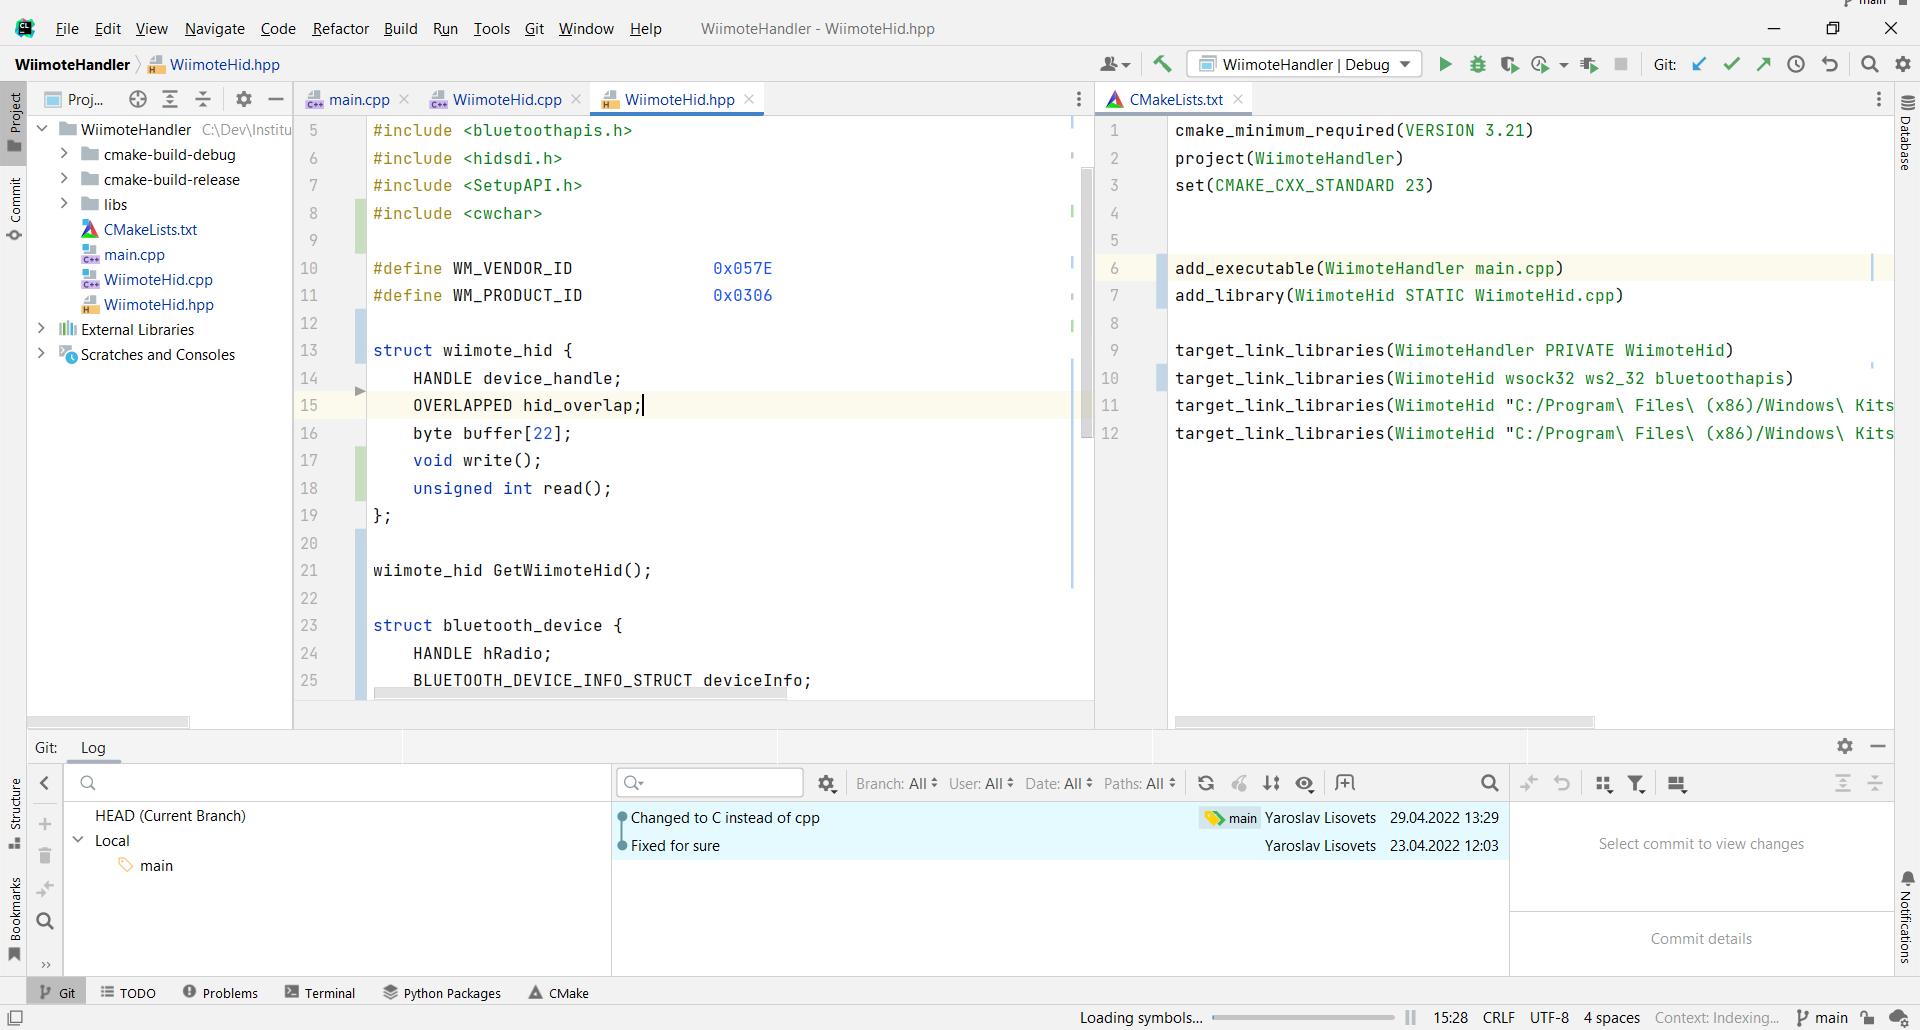
\includegraphics[width=\textwidth]{content/clion_screenshot}
\captionof{figure}{Скриншот из Clion с открытыми окнами редактирования заголовочного файла и файла CMake }

\subsubsection{IntelliJ Rust}
\quad IntelliJ Rust\footnote{плагин с открытым исходным кодом совместимый со всеми IDE основанными на IntelliJ IDEA для Rust.\href{ https://plugins.jetbrains.com/plugin/8182-rust}{https://plugins.jetbrains.com/plugin/8182-rust}}
- плагин с открытым исходным кодом совместимый со всеми IDE основанными на IntelliJ IDEA\@.
В паре с IntelliJ TOML  \footnote{IntelliJ TOML \href{ https://plugins.jetbrains.com/plugin/8195-toml}{https://plugins.jetbrains.com/plugin/8195-toml}} он направлен на то, чтобы привнести полный опыт IDE в ваш рабочий процесс с Rust и Cargo.

\subsubsection{CMake}
\quad \text{CMake\footnote{Семейство инструментов CMake \href{https://cmake.org/}{https://cmake.org/}}
 - это семейство} инструментов с открытым исходным кодом для создания, тестирования программного обеспечения.
 CMake используется для управления процессом компиляции программного обеспечения с помощью простых файлов конфигурации,
 независимых от платформы и компилятора.

\section{Создание приложения}

\subsection{Состав и Характеристики файлов проекта}
\begin{table}[!h]
    \centering
    \begin{tabular}{p{0.35\linewidth} | p{0.6\linewidth}|}
        \hline
        \multicolumn{2}{|l|}{Заголовочные файлы} \\ \hline
        \multicolumn{1}{|l|}{WiimoteHid.hpp} & Основной заголовочный файл проекта, подключающий внешние заголовочные файлы и необходимый для работы с библиотекой.
        Также в нём происходит объявление функций библиотеки. \\ \hline
        \multicolumn{2}{|l|}{Файлы исходного кода} \\ \hline
        \multicolumn{1}{|l|}{WiimoteHid.сpp} & Содержит реализацию функций объявленных в WiimoteHid.hpp \\ \hline
        \multicolumn{1}{|l|}{lib.rs} & Является абстракцией над библиотекой для предоставления упрощённого интерфейса взаимодействия с геймпадом Wiimote \\ \hline
        \multicolumn{2}{|l|}{Вспомогательные файлы} \\ \hline
        \multicolumn{1}{|l|}{bindings.rs} & Сгенерированные из WiimoteHid.hpp с помощью инструмента bindgen.
        Необходим для компиляции lib.rs. \\ \hline
    \end{tabular}
    \caption{\label{tab:table-name}Описание файлов проекта}
\end{table}
\subsection{Стандартные классы и функции приложения}
\begin{tabularx}{\linewidth}{|X|X|X|}
    \hline
        Название & Назначение & Параметры \\ \hline
        BluetoothFindFirstRadio & Получение handle'а к bluetooth модулю.
        & Принимает указатель на структуру с параметрами, по которым будет вестись поиск, а так же указатель на handle. \\ \hline
        BluetoothFindNextRadio & Возвращает handle к следующему bluetooth модулю, если тот имеется.
        & Принимает handle на предыдущий модуль, и handle куда будет записан новый в случае нахождения. \\ \hline
        BluetoothGetRadioInfo & Получение данных таких, как адрес, имя, класс устройства и информации производителя, о bluetooth модуле.
        & Принимает структуру, в которую будет записана информация, и handle к модулю. \\ \hline
        BluetoothFindFirstDevice & Получение handle'а первого найденного устройства в зоне действия bluetooth модуля.
        & Принимает структуру, куда будет записана информация о найденном устройстве, и параметрами, по которым будет вестись поиск. \\ \hline
        BluetoothFindNextDevice & Получение handle'а следующего найденного устройства.
        & Принимает структуру, куда будет записана информация о найденном устройстве, и параметрами, по которым будет вестись поиск. \\ \hline
        CloseHandle & Закрывает(возвращает системе) handle.
        & Принимает handle, который планируется закрыть. \\ \hline
        wcscmp & Возвращает разницу между переданными строками.
        & Принимает два указателя на wchar\_t \\ \hline
        BluetoothRemoveDevice & Удаляет устройство из списка прежде подключённых в операционной.
        & Принимает адрес устройства, которое надо удалить. \\ \hline
        BluetoothSetServiceState & Устанавливает состояние bluetooth сервиса Windows, например для указания сопряжения с устройством.
        & Принимает handle к bluetooth модулю, информации об устройстве, ID сервиса, через который будет происходить работа, устанавливаемое состояние. \\ \hline
        HidD\_GetHidGuid & Получение id для HID сервиса.
        & Принимает ссылку на переменную куда будет записан id. \\ \hline
        SetupDiGetClassDevs & Функция возвращает дескриптор набора информации об устройстве, который содержит запрошенные элементы информации.
        & Принимает указатель на устройство, счётчик, handle к окну и флаги. \\ \hline
        SetupDiEnumDeviceInterfaces & Функция SetupDiEnumDeviceInterfaces перечисляет интерфейсы устройств, которые содержатся в наборе информации об устройстве.
        & Принимает DeviceInfoSet, DeviceInfoData, ID устройства, индекс, переменную куда будут записаны данные. \\ \hline
        HidD\_GetAttributes & Возвращает атрибуты переданного устройства.
        & Получает handle устройства, и ссылку на структуру, куда будут записаны дынные. \\ \hline
        CreateEvent & Служит для создания объекта события.
        & Получает указатель на структуру SECURITY\_ATTRIBUTES, булевую переменную устанавливающую автоматический или ручной перезапуск, булевое начальное состояние, имя события. \\ \hline
        ResetEvent & Перезапускает событие.
        & Получает ссылку на событие. \\ \hline
        WriteFile & Записывает данные в указанный файл или устройство ввода/вывода (I/O).
        & Получает handle куда будет производиться запись, указатель на записываемые данные, количество записываемых байтов, ссылка на переменную куда будет записано количество отправленных байтов, указатель на переменную, которая содержит информацию, используемую при асинхронном (или перекрывающемся) вводе и выводе. \\ \hline
        ReadFile & Считывает данные из указанного файла или устройства ввода/вывода (I/O).
        & Получает handle устройства/файла, указатель на буфер куда будут прочитаны данные, количество считываемых байтов, ссылка на переменную куда будет записано количество полученных байтов, указатель на переменную, которая содержит информацию, используемую при асинхронном (или перекрывающемся) вводе и выводе. \\ \hline
        WaitForSingleObject & Ожидает событие в течение указанного времени.
        & Получает указатель на событие. \\ \hline
        CancelIo & Отменяет ожидания ввода и вывода для устройства/файла.
        & Получает дескриптор устройства. \\ \hline
        GetOverlappedResult & Извлекает результаты перекрывающейся/асинхронной операции с указанным файлом, или устройством, или именованным каналом.
        & Получает дескриптор устройства, ссылку на OVERLAPPED, ссылку на переменную куда будет записано количество прочитанных байтов, время ожидания. \\ \hline
        \caption{\label{tab:table} Таблица с описанием стандартных использованных функций}
\end{tabularx}
\subsection{Пользовательские структуры в приложении}
\subsubsection{struct wiimote\_hid}
\quad Необходима для хранения:\\
\quad Hid дескриптора, через который происходит обращение к устройству\\
\quad Переменной типа OVERLAPPED, предназначенной синхронизации с потоками ввода и вывода\\
\quad Буфера, используемого при чтении и записи.\\
Через данную структуру происходит получение и отправка данных.
Для этого содержит методы чтения и записи.

\subsubsection{struct bluetooth\_device}
\quad В данной структуре хранится HANDLE к bluetooth модулю и BLUETOOTH\_DEVICE\_INFO\_STRUCT, с помощью которого происходит обращение к устройству.


\subsection{Пользовательские функции в приложении}
\subsubsection{wiimote\_hid::write()}
\quad Предназначена для записи данных из буфера структуры wiimote\_hid.

\subsubsection{wiimote\_hid::read()}
\quad Предназначена для записи данных в буфер структуры wiimote\_hid.
Возвращает количество прочитанных байтов.

\subsubsection{GetWiimoteHid()}
\quad Производит поиск геймпада среди подключённых hid устройств и при нахождении устанавливает с ним соединение.\\
\quad Возвращает структуру wiimote\_hid.

\subsubsection{void ProcessWiimotes(bool new\_scan, const T \&callback = nullptr)}
\quad Производит поиск bluetooth устройств.
При нахождении такого производит вызов callback функцию, устанавливающую соединение.

\subsubsection{bool AttachWiimote(HANDLE hRadio, const BLUETOOTH\_RADIO\_INFO \&radio\_info, BLUETOOTH\_DEVICE\_INFO\_STRUCT \&deviceInfo)}
\quad Устанавливает соединение с геймпадом.

\subsubsection{bool ForgetWiimote(BLUETOOTH\_DEVICE\_INFO\_STRUCT \&deviceInfo)}
\quad Производит удаление удаление устройства из списка операционной системы с ранее подключёнными устройствами.

\subsubsection{void wiimoteDisconnect(bluetooth\_device *bluetoothDevice)}
\quad Разрывает bluetooth соединение с геймпадом.

\subsubsection{bluetooth\_device *FindConnectWiimoteBLE()}
\quad Производит цикл поиска и подключения к устройству и возвращает структуру с дескриптором к bluetooth модулю и информацией о bluetooth-устройстве.
\newcommand{\centered}[1]{\begin{tabular}{l} #1 \end{tabular}}
\subsection{Пользовательские функции в приложении}
\begin{tabularx}{\linewidth}{|X|X|}
    \hline
    wiimote\_hid::write& Предназначена для записи данных из буфера структуры wiimote\_hid.\\\hline

    wiimote\_hid::read& Предназначена для записи данных в буфер структуры wiimote\_hid.Возвращает количество прочитанных байтов.\\\hline

    GetWiimoteHid& Производит поиск геймпада среди подключённых hid устройств и при нахождении устанавливает с ним соединение.
    Возвращает структуру wiimote\_hid.\\\hline

    void ProcessWiimotes& Производит поиск bluetooth устройств.При нахождении такого производит вызов callback функцию, устанавливающую соединение.\\\hline

    bool AttachWiimote& Устанавливает соединение с геймпадом.\\\hline

    bool ForgetWiimote& Производит удаление удаление устройства из списка операционной системы с ранее подключёнными устройствами.\\\hline

    void wiimoteDisconnect& Разрывает bluetooth соединение с геймпадом.\\\hline

    bluetooth\_device *FindConnectWiimoteBLE& Производит цикл поиска и подключения к устройству и возвращает структуру с дескриптором к bluetooth модулю и информацией о bluetooth-устройстве.\\\hline
\end{tabularx}

\subsection{Структура программы}
    \begin{center}
        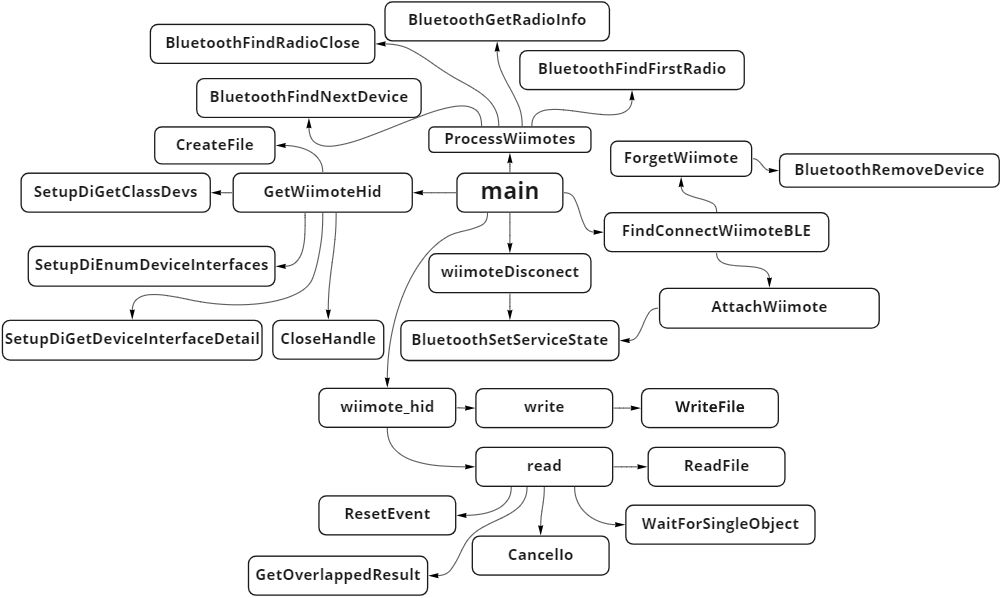
\includegraphics[width=\textwidth]{content/program_structure}

        \captionof{figure}{Структура программы}
    \end{center}

\subsection{Системные требования}
\begin{enumerate}
    \item Семейство операционных систем Windows.
    \item Наличие свободного места в размере 158кб.
    \item Bluetooth модуль.
    \item Геймпад от Nintendo Wii - Wiimote.
\end{enumerate}




\section{Руководство по использованию}
\quad {Для начала работы необходимо запустить программу}.
Для этого не обходимо нажать два раза по иконке приложения или выделить и уже после этого нажать клавишу enter.\\
\quad {После} запуска в консоли появится сообщение о необходимости нажатия кнопок 1 и 2 для перевода геймпада в режим синхронизации.
Также есть альтернатива в виде нажатия отельной кнопки синхронизации в отсеке с аккумуляторами.
После чего должна пройти синхронизация.
В случае успешного установления синхронизации будет выведено сообщение, оповещающее пользователя об этом.
\quad Совместно с этим сообщением будет выведена инструкция о работе с геймпадом.\\
\quad Инструкция:\\
\begin{itemize}
    \item Нажимайте кнопки 1 или 2 для изменения состояния светодиодного индикатора.
    \item Нажмите B для включения/отключения вибрации.
    \item Нажмите A, чтобы включить/отключить акселерометр.
    \item {Одновременно нажмите A и Минус, чтобы отключить геймпад.}
\end{itemize}
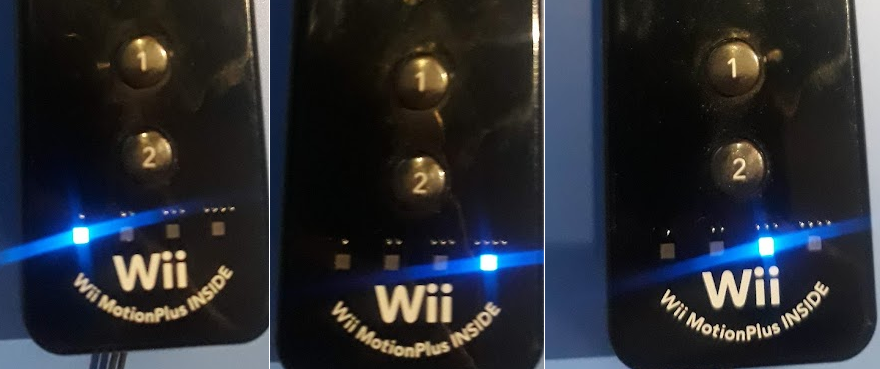
\includegraphics[width=\textwidth]{content/LedsChange}
\captionof{figure}{Пример переключения светодиодов с помощью клавиш 1 и 2}
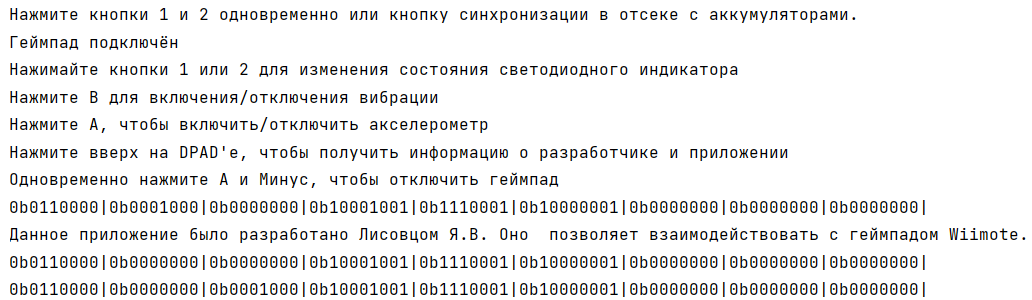
\includegraphics[width=\textwidth]{content/ProgramOutput}
\captionof{figure}{Пример работы программы}



\lstset { %
    language=C++,
    backgroundcolor=\color{white!5}, % set backgroundcolor
    basicstyle=\footnotesize,
    breaklines=true,
    postbreak=\mbox{\textcolor{black}{$\hookrightarrow$}\space},
    showstringspaces=false,
    extendedchars=\true
}

\edef\@currentlabel{Список литературы}
\renewcommand{\footnotesize}{\fontsize{9pt}{11pt}\selectfont}
\raggedright


\printendnotes
\newpage
\newgeometry{right = 0.5in, left=0.5in, top=1in, bottom=0.5in}
\lstset{basicstyle=\footnotesize, columns=fullflexible}
\section{Приложение 1. Исходный тексты программы}
\subsection{WiimoteHid.hpp}
\lstinputlisting{..//WiimoteHandler/WiimoteHid.hpp}
\subsection{WiimoteHid.cpp}
\lstinputlisting{../WiimoteHandler/WiimoteHid.cpp}
\lstset { language=Rust}
\lstdefinelanguage{Rust}{morestring=[b]"}
\subsection{main.rs}
\lstinputlisting{../Wiimote/src/main.rs}
\subsection{lib.rs}
\lstinputlisting{../Wiimote/src/lib.rs}
\section{Приложение 2. Алгоритмы функций }
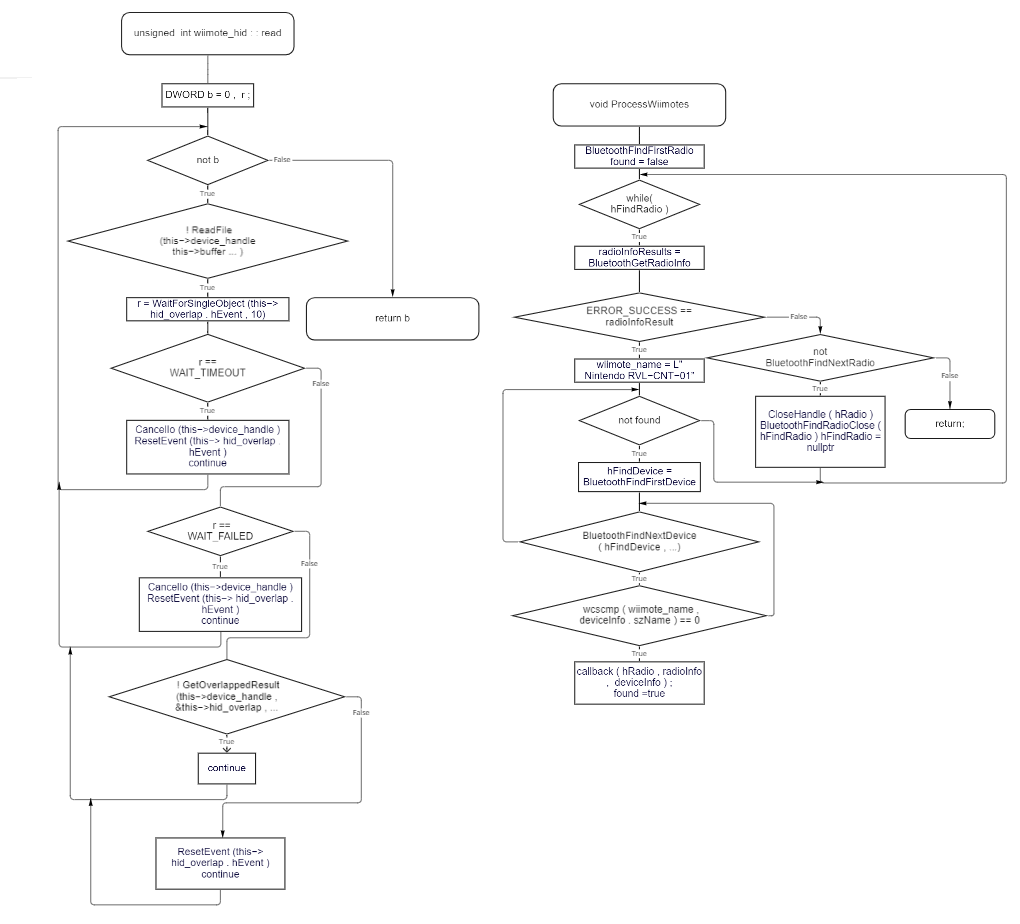
\includegraphics[width=\textwidth]{content/Algorithm}
\caption{Алгоритмы функций wiimote::read и ProcessWiimotes}


\end{document}